\documentclass[twoside]{book}

% Packages required by doxygen
\usepackage{fixltx2e}
\usepackage{calc}
\usepackage{doxygen}
\usepackage{graphicx}
\usepackage[utf8]{inputenc}
\usepackage{makeidx}
\usepackage{multicol}
\usepackage{multirow}
\PassOptionsToPackage{warn}{textcomp}
\usepackage{textcomp}
\usepackage[nointegrals]{wasysym}
\usepackage[table]{xcolor}

% Font selection
\usepackage[T1]{fontenc}
\usepackage{mathptmx}
\usepackage[scaled=.90]{helvet}
\usepackage{courier}
\usepackage{amssymb}
\usepackage{sectsty}
\renewcommand{\familydefault}{\sfdefault}
\allsectionsfont{%
  \fontseries{bc}\selectfont%
  \color{darkgray}%
}
\renewcommand{\DoxyLabelFont}{%
  \fontseries{bc}\selectfont%
  \color{darkgray}%
}
\newcommand{\+}{\discretionary{\mbox{\scriptsize$\hookleftarrow$}}{}{}}

% Page & text layout
\usepackage{geometry}
\geometry{%
  a4paper,%
  top=2.5cm,%
  bottom=2.5cm,%
  left=2.5cm,%
  right=2.5cm%
}
\tolerance=750
\hfuzz=15pt
\hbadness=750
\setlength{\emergencystretch}{15pt}
\setlength{\parindent}{0cm}
\setlength{\parskip}{0.2cm}
\makeatletter
\renewcommand{\paragraph}{%
  \@startsection{paragraph}{4}{0ex}{-1.0ex}{1.0ex}{%
    \normalfont\normalsize\bfseries\SS@parafont%
  }%
}
\renewcommand{\subparagraph}{%
  \@startsection{subparagraph}{5}{0ex}{-1.0ex}{1.0ex}{%
    \normalfont\normalsize\bfseries\SS@subparafont%
  }%
}
\makeatother

% Headers & footers
\usepackage{fancyhdr}
\pagestyle{fancyplain}
\fancyhead[LE]{\fancyplain{}{\bfseries\thepage}}
\fancyhead[CE]{\fancyplain{}{}}
\fancyhead[RE]{\fancyplain{}{\bfseries\leftmark}}
\fancyhead[LO]{\fancyplain{}{\bfseries\rightmark}}
\fancyhead[CO]{\fancyplain{}{}}
\fancyhead[RO]{\fancyplain{}{\bfseries\thepage}}
\fancyfoot[LE]{\fancyplain{}{}}
\fancyfoot[CE]{\fancyplain{}{}}
\fancyfoot[RE]{\fancyplain{}{\bfseries\scriptsize Generated on Fri Mar 25 2016 03\+:15\+:43 for C++ Templates by Doxygen }}
\fancyfoot[LO]{\fancyplain{}{\bfseries\scriptsize Generated on Fri Mar 25 2016 03\+:15\+:43 for C++ Templates by Doxygen }}
\fancyfoot[CO]{\fancyplain{}{}}
\fancyfoot[RO]{\fancyplain{}{}}
\renewcommand{\footrulewidth}{0.4pt}
\renewcommand{\chaptermark}[1]{%
  \markboth{#1}{}%
}
\renewcommand{\sectionmark}[1]{%
  \markright{\thesection\ #1}%
}

% Indices & bibliography
\usepackage{natbib}
\usepackage[titles]{tocloft}
\setcounter{tocdepth}{3}
\setcounter{secnumdepth}{5}
\makeindex

% Hyperlinks (required, but should be loaded last)
\usepackage{ifpdf}
\ifpdf
  \usepackage[pdftex,pagebackref=true]{hyperref}
\else
  \usepackage[ps2pdf,pagebackref=true]{hyperref}
\fi
\hypersetup{%
  colorlinks=true,%
  linkcolor=blue,%
  citecolor=blue,%
  unicode%
}

% Custom commands
\newcommand{\clearemptydoublepage}{%
  \newpage{\pagestyle{empty}\cleardoublepage}%
}


%===== C O N T E N T S =====

\begin{document}

% Titlepage & ToC
\hypersetup{pageanchor=false,
             bookmarks=true,
             bookmarksnumbered=true,
             pdfencoding=unicode
            }
\pagenumbering{roman}
\begin{titlepage}
\vspace*{7cm}
\begin{center}%
{\Large C++ Templates }\\
\vspace*{1cm}
{\large Generated by Doxygen 1.8.8}\\
\vspace*{0.5cm}
{\small Fri Mar 25 2016 03:15:43}\\
\end{center}
\end{titlepage}
\clearemptydoublepage
\tableofcontents
\clearemptydoublepage
\pagenumbering{arabic}
\hypersetup{pageanchor=true}

%--- Begin generated contents ---
\chapter{Hierarchical Index}
\section{Class Hierarchy}
This inheritance list is sorted roughly, but not completely, alphabetically\+:\begin{DoxyCompactList}
\item \contentsline{section}{Array\+Base$<$ T $>$}{\pageref{d8/d84/a00001}}{}
\begin{DoxyCompactList}
\item \contentsline{section}{Dynamic\+Array$<$ T $>$}{\pageref{d7/d46/a00002}}{}
\end{DoxyCompactList}
\end{DoxyCompactList}

\chapter{Class Index}
\section{Class List}
Here are the classes, structs, unions and interfaces with brief descriptions\+:\begin{DoxyCompactList}
\item\contentsline{section}{\hyperlink{a00001}{Array\+Base$<$ T $>$} \\*Base class for array-\/like structures }{\pageref{d8/d84/a00001}}{}
\item\contentsline{section}{\hyperlink{a00002}{Dynamic\+Array$<$ T $>$} \\*A resizable array. Inherits \hyperlink{a00001}{Array\+Base} }{\pageref{d7/d46/a00002}}{}
\end{DoxyCompactList}

\chapter{File Index}
\section{File List}
Here is a list of all files with brief descriptions\+:\begin{DoxyCompactList}
\item\contentsline{section}{/home/bdfoster/\+Projects/c++/templates/\hyperlink{a00003}{Array\+Base.\+cpp} }{\pageref{d1/d7c/a00003}}{}
\item\contentsline{section}{/home/bdfoster/\+Projects/c++/templates/\hyperlink{a00004}{Array\+Base.\+h} }{\pageref{d0/d0b/a00004}}{}
\item\contentsline{section}{/home/bdfoster/\+Projects/c++/templates/\hyperlink{a00005}{Dynamic\+Array.\+cpp} }{\pageref{dd/dad/a00005}}{}
\item\contentsline{section}{/home/bdfoster/\+Projects/c++/templates/\hyperlink{a00006}{Dynamic\+Array.\+h} }{\pageref{de/d21/a00006}}{}
\end{DoxyCompactList}

\chapter{Class Documentation}
\hypertarget{a00001}{\section{Array\+Base$<$ T $>$ Class Template Reference}
\label{a00001}\index{Array\+Base$<$ T $>$@{Array\+Base$<$ T $>$}}
}


Base class for array-\/like structures.  




{\ttfamily \#include $<$Array\+Base.\+h$>$}



Inheritance diagram for Array\+Base$<$ T $>$\+:
\nopagebreak
\begin{figure}[H]
\begin{center}
\leavevmode
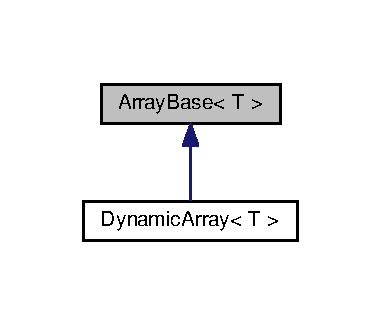
\includegraphics[width=183pt]{d7/d7a/a00016}
\end{center}
\end{figure}
\subsection*{Public Types}
\begin{DoxyCompactItemize}
\item 
typedef T \hyperlink{a00001_aa881b5ee704e0f293b4dddbaf8990149}{type}
\end{DoxyCompactItemize}
\subsection*{Public Member Functions}
\begin{DoxyCompactItemize}
\item 
\hyperlink{a00001_a949fbe49f202aed7d4ce8442b7fd0bd5}{Array\+Base} (void)
\item 
\hyperlink{a00001_af9db2c439a3c5bc723c66d44ba4049a0}{Array\+Base} (size\+\_\+t max\+Size)
\item 
\hyperlink{a00001_a5de8eae891c4d4f855a6739fc573de85}{Array\+Base} (size\+\_\+t max\+Size, T \hyperlink{a00001_a6becc5e91c79d7693c0d406e466f9ec6}{fill})
\item 
\hyperlink{a00001_a76eb6a2544ace5a6c8cc972b876b60a0}{$\sim$\+Array\+Base} (void)
\item 
size\+\_\+t \hyperlink{a00001_aeed263e1e987901c8cc2c1e1d3102d73}{size} (void)
\item 
T \hyperlink{a00001_aabda9501caf50b75ce09e7ef47fd1de7}{get} (size\+\_\+t index) const 
\item 
void \hyperlink{a00001_a5a9fe61509061defe530d0ebc3a91497}{set} (size\+\_\+t index, T contents)
\item 
int \hyperlink{a00001_adc718f38281ba844303941c4d111cc8c}{find} (T element)
\item 
int \hyperlink{a00001_a450ec98ae75a13f7dfbd6ba499218b8e}{find} (T element, size\+\_\+t start\+Index)
\item 
void \hyperlink{a00001_a6becc5e91c79d7693c0d406e466f9ec6}{fill} (T contents)
\item 
void \hyperlink{a00001_a11dc3b617f2fedbb3b499971493b9c4f}{clear} ()
\item 
virtual bool \hyperlink{a00001_a1687635b3bda64e9064e53b8d5a91ac1}{is\+Empty} ()
\item 
bool \hyperlink{a00001_a95a446bcd6e8b2ff10e6f5c0232e6069}{operator==} (const \hyperlink{a00001}{Array\+Base}$<$ T $>$ \&rhs) const 
\item 
bool \hyperlink{a00001_acb1f14f8761d00708f25281854bf0769}{operator!=} (const \hyperlink{a00001}{Array\+Base}$<$ T $>$ \&rhs) const 
\item 
T \hyperlink{a00001_a654b9073ee55e973fc31a9c03affe423}{operator\mbox{[}$\,$\mbox{]}} (size\+\_\+t index) const 
\item 
T \& \hyperlink{a00001_a38d83584b9e023781779af9dd733d822}{operator\mbox{[}$\,$\mbox{]}} (size\+\_\+t index)
\end{DoxyCompactItemize}


\subsection{Detailed Description}
\subsubsection*{template$<$typename T$>$class Array\+Base$<$ T $>$}

Base class for array-\/like structures. 

Contains the actual raw array of type T along with common properties and methods for array like structures. \begin{DoxySince}{Since}
0.\+1.\+0 
\end{DoxySince}

\begin{DoxyTemplParams}{Template Parameters}
{\em T} & (typename) Element type of array. \\
\hline
\end{DoxyTemplParams}


Definition at line 22 of file Array\+Base.\+h.



\subsection{Member Typedef Documentation}
\hypertarget{a00001_aa881b5ee704e0f293b4dddbaf8990149}{\index{Array\+Base@{Array\+Base}!type@{type}}
\index{type@{type}!Array\+Base@{Array\+Base}}
\subsubsection[{type}]{\setlength{\rightskip}{0pt plus 5cm}template$<$typename T $>$ typedef T {\bf Array\+Base}$<$ T $>$\+::{\bf type}}}\label{a00001_aa881b5ee704e0f293b4dddbaf8990149}


Definition at line 46 of file Array\+Base.\+h.



\subsection{Constructor \& Destructor Documentation}
\hypertarget{a00001_a949fbe49f202aed7d4ce8442b7fd0bd5}{\index{Array\+Base@{Array\+Base}!Array\+Base@{Array\+Base}}
\index{Array\+Base@{Array\+Base}!Array\+Base@{Array\+Base}}
\subsubsection[{Array\+Base}]{\setlength{\rightskip}{0pt plus 5cm}template$<$typename T $>$ {\bf Array\+Base}$<$ T $>$\+::{\bf Array\+Base} (
\begin{DoxyParamCaption}
\item[{void}]{}
\end{DoxyParamCaption}
)}}\label{a00001_a949fbe49f202aed7d4ce8442b7fd0bd5}
Default initializing constructor.

Creates the raw array of type {\ttfamily T} and sets the maximum size to 10 by default. 

Definition at line 17 of file Array\+Base.\+cpp.


\begin{DoxyCode}
17                              :
18     \_data (\textcolor{keyword}{new} T[10]),
19     \_currentSize (0),
20     \_maxSize (10) \{ \}
\end{DoxyCode}
\hypertarget{a00001_af9db2c439a3c5bc723c66d44ba4049a0}{\index{Array\+Base@{Array\+Base}!Array\+Base@{Array\+Base}}
\index{Array\+Base@{Array\+Base}!Array\+Base@{Array\+Base}}
\subsubsection[{Array\+Base}]{\setlength{\rightskip}{0pt plus 5cm}template$<$typename T $>$ {\bf Array\+Base}$<$ T $>$\+::{\bf Array\+Base} (
\begin{DoxyParamCaption}
\item[{size\+\_\+t}]{max\+Size}
\end{DoxyParamCaption}
)}}\label{a00001_af9db2c439a3c5bc723c66d44ba4049a0}
Initializing constructor. Sets max size to {\ttfamily max\+Size}, effectively overriding the default.


\begin{DoxyParams}{Parameters}
{\em max\+Size} & (size\+\_\+t) Maximum size of the array. \\
\hline
\end{DoxyParams}


Definition at line 26 of file Array\+Base.\+cpp.


\begin{DoxyCode}
26                                        :
27     \_data (\textcolor{keyword}{nullptr}),
28     \_currentSize (0),
29     \_maxSize (0)
30 \{
31     \textcolor{keywordflow}{if} (maxSize > 0) \{
32         this->\_maxSize = maxSize;
33     \} \textcolor{keywordflow}{else} \{
34         this->\_maxSize = 10;
35     \}
36     
37     this->\_data = \textcolor{keyword}{new} T[this->\_maxSize];
38 \}
\end{DoxyCode}
\hypertarget{a00001_a5de8eae891c4d4f855a6739fc573de85}{\index{Array\+Base@{Array\+Base}!Array\+Base@{Array\+Base}}
\index{Array\+Base@{Array\+Base}!Array\+Base@{Array\+Base}}
\subsubsection[{Array\+Base}]{\setlength{\rightskip}{0pt plus 5cm}template$<$typename T $>$ {\bf Array\+Base}$<$ T $>$\+::{\bf Array\+Base} (
\begin{DoxyParamCaption}
\item[{size\+\_\+t}]{max\+Size, }
\item[{T}]{fill}
\end{DoxyParamCaption}
)}}\label{a00001_a5de8eae891c4d4f855a6739fc573de85}
Initializing constructor. Sets max size to {\ttfamily max\+Size} and filling each element of the array with {\ttfamily fill}.


\begin{DoxyParams}{Parameters}
{\em max\+Size} & (size\+\_\+t) Maximum size of the array. \\
\hline
{\em fill} & (T) Contents of each element. \\
\hline
\end{DoxyParams}


Definition at line 44 of file Array\+Base.\+cpp.


\begin{DoxyCode}
44                                                :
45     \_data (\textcolor{keyword}{nullptr}),
46     \_currentSize (0),
47     \_maxSize (0)
48 \{
49     \textcolor{keywordflow}{if} (maxSize > 0) \{
50         this->\_maxSize = maxSize;
51     \} \textcolor{keywordflow}{else} \{
52         this->\_maxSize = 10;
53     \}
54 
55     this->\_data = \textcolor{keyword}{new} T[this->\_maxSize];
56 
57     this->\hyperlink{a00001_a6becc5e91c79d7693c0d406e466f9ec6}{fill}(\hyperlink{a00001_a6becc5e91c79d7693c0d406e466f9ec6}{fill});
58 \}
\end{DoxyCode}
\hypertarget{a00001_a76eb6a2544ace5a6c8cc972b876b60a0}{\index{Array\+Base@{Array\+Base}!````~Array\+Base@{$\sim$\+Array\+Base}}
\index{````~Array\+Base@{$\sim$\+Array\+Base}!Array\+Base@{Array\+Base}}
\subsubsection[{$\sim$\+Array\+Base}]{\setlength{\rightskip}{0pt plus 5cm}template$<$typename T $>$ {\bf Array\+Base}$<$ T $>$\+::$\sim${\bf Array\+Base} (
\begin{DoxyParamCaption}
\item[{void}]{}
\end{DoxyParamCaption}
)}}\label{a00001_a76eb6a2544ace5a6c8cc972b876b60a0}
Destructor

\begin{DoxySince}{Since}
0.\+1.\+0 
\end{DoxySince}


Definition at line 64 of file Array\+Base.\+cpp.


\begin{DoxyCode}
65 \{
66     \textcolor{comment}{// Only delete if this->\_data isn't a nullptr.}
67     \textcolor{keywordflow}{if} (\textcolor{keyword}{nullptr} != this->\_data) \{
68         \textcolor{keyword}{delete} [] this->\_data;
69     \}
70 \}
\end{DoxyCode}


\subsection{Member Function Documentation}
\hypertarget{a00001_a11dc3b617f2fedbb3b499971493b9c4f}{\index{Array\+Base@{Array\+Base}!clear@{clear}}
\index{clear@{clear}!Array\+Base@{Array\+Base}}
\subsubsection[{clear}]{\setlength{\rightskip}{0pt plus 5cm}template$<$typename T $>$ void {\bf Array\+Base}$<$ T $>$\+::clear (
\begin{DoxyParamCaption}
{}
\end{DoxyParamCaption}
)}}\label{a00001_a11dc3b617f2fedbb3b499971493b9c4f}
Clears all elements from the array. \begin{DoxyReturn}{Returns}
(void) 
\end{DoxyReturn}
\begin{DoxySince}{Since}
0.\+1.\+0 
\end{DoxySince}
\hypertarget{a00001_a6becc5e91c79d7693c0d406e466f9ec6}{\index{Array\+Base@{Array\+Base}!fill@{fill}}
\index{fill@{fill}!Array\+Base@{Array\+Base}}
\subsubsection[{fill}]{\setlength{\rightskip}{0pt plus 5cm}template$<$typename T $>$ void {\bf Array\+Base}$<$ T $>$\+::fill (
\begin{DoxyParamCaption}
\item[{T}]{contents}
\end{DoxyParamCaption}
)}}\label{a00001_a6becc5e91c79d7693c0d406e466f9ec6}
Set each element in raw array to given {\ttfamily element} up to the maximum size.


\begin{DoxyParams}{Parameters}
{\em contents} & (T) Element to fill \hyperlink{a00001}{Array\+Base} with. \\
\hline
\end{DoxyParams}
\begin{DoxyReturn}{Returns}
(void) 
\end{DoxyReturn}
\begin{DoxySince}{Since}
0.\+1.\+0 
\end{DoxySince}


Definition at line 158 of file Array\+Base.\+cpp.


\begin{DoxyCode}
159 \{
160     \textcolor{comment}{// For each element in the array, assign to contents.}
161     \textcolor{keywordflow}{for} (\textcolor{keywordtype}{size\_t} i = 0; i < this->\_maxSize; i++) \{
162         this->\_data[i] = contents;
163     \}
164 
165     this->\_currentSize = this->\_maxSize;
166 \}
\end{DoxyCode}
\hypertarget{a00001_adc718f38281ba844303941c4d111cc8c}{\index{Array\+Base@{Array\+Base}!find@{find}}
\index{find@{find}!Array\+Base@{Array\+Base}}
\subsubsection[{find}]{\setlength{\rightskip}{0pt plus 5cm}template$<$typename T $>$ int {\bf Array\+Base}$<$ T $>$\+::find (
\begin{DoxyParamCaption}
\item[{T}]{element}
\end{DoxyParamCaption}
)}}\label{a00001_adc718f38281ba844303941c4d111cc8c}
Return first {\ttfamily index} that matches element.


\begin{DoxyParams}{Parameters}
{\em element} & (T) Element to match with. \\
\hline
\end{DoxyParams}
\begin{DoxyReturn}{Returns}
(int) {\ttfamily index} or -\/1 if no match. 
\end{DoxyReturn}
\begin{DoxySince}{Since}
0.\+1.\+0 
\end{DoxySince}


Definition at line 115 of file Array\+Base.\+cpp.


\begin{DoxyCode}
116 \{
117     \textcolor{keywordflow}{return} this->\hyperlink{a00001_adc718f38281ba844303941c4d111cc8c}{find}(element, 0);
118 \}
\end{DoxyCode}
\hypertarget{a00001_a450ec98ae75a13f7dfbd6ba499218b8e}{\index{Array\+Base@{Array\+Base}!find@{find}}
\index{find@{find}!Array\+Base@{Array\+Base}}
\subsubsection[{find}]{\setlength{\rightskip}{0pt plus 5cm}template$<$typename T $>$ int {\bf Array\+Base}$<$ T $>$\+::find (
\begin{DoxyParamCaption}
\item[{T}]{element, }
\item[{size\+\_\+t}]{start\+Index}
\end{DoxyParamCaption}
)}}\label{a00001_a450ec98ae75a13f7dfbd6ba499218b8e}
Return first {\ttfamily index} that matches {\ttfamily element} starting at the given index.


\begin{DoxyParams}{Parameters}
{\em element} & (T) Element to match with. \\
\hline
{\em start\+Index} & (size\+\_\+t) The {\ttfamily index} to start with. \\
\hline
\end{DoxyParams}
\begin{DoxyReturn}{Returns}
(int) {\ttfamily index} or -\/1 if no match. 
\end{DoxyReturn}
\begin{DoxySince}{Since}
0.\+1.\+0 
\end{DoxySince}


Definition at line 124 of file Array\+Base.\+cpp.


\begin{DoxyCode}
125 \{
126     \textcolor{comment}{/* Check to make sure index is within range.}
127 \textcolor{comment}{     * If not, throw std::out\_of\_range exception.}
128 \textcolor{comment}{     */}
129     \textcolor{keywordflow}{if} (startIndex >= this->\_currentSize) \{
130         \textcolor{comment}{// index is out of range}
131         \textcolor{keywordflow}{throw} std::out\_of\_range(\textcolor{stringliteral}{"Invalid index value"});
132     \}
133 
134     \textcolor{keywordtype}{int} returnIndex = -1;
135 
136     \textcolor{comment}{/*}
137 \textcolor{comment}{     * While returnIndex equals -1 and start is less than }
138 \textcolor{comment}{     * \_currentSize, keep going.}
139 \textcolor{comment}{     */}
140     \textcolor{keywordflow}{while} (returnIndex == -1 && startIndex < this->\_currentSize) \{
141         \textcolor{comment}{// Check to see if data at current startIndex equals element.}
142         \textcolor{keywordflow}{if} (this->\_data[startIndex] == element) \{
143             \textcolor{comment}{// Match, set startIndex as returnIndex, loop completes.}
144             returnIndex == startIndex;
145         \} \textcolor{keywordflow}{else} \{
146             \textcolor{comment}{// No match, increment startIndex}
147             startIndex++;
148         \}
149     \}
150 
151     \textcolor{keywordflow}{return} returnIndex;
152 \}
\end{DoxyCode}
\hypertarget{a00001_aabda9501caf50b75ce09e7ef47fd1de7}{\index{Array\+Base@{Array\+Base}!get@{get}}
\index{get@{get}!Array\+Base@{Array\+Base}}
\subsubsection[{get}]{\setlength{\rightskip}{0pt plus 5cm}template$<$typename T $>$ T {\bf Array\+Base}$<$ T $>$\+::get (
\begin{DoxyParamCaption}
\item[{size\+\_\+t}]{index}
\end{DoxyParamCaption}
) const}}\label{a00001_aabda9501caf50b75ce09e7ef47fd1de7}
Query the element at specified index.


\begin{DoxyParams}{Parameters}
{\em index} & (size\+\_\+t) Index of query element. \\
\hline
\end{DoxyParams}
\begin{DoxyReturn}{Returns}
(T) The element at specified index. 
\end{DoxyReturn}

\begin{DoxyExceptions}{Exceptions}
{\em std\+::out\+\_\+of\+\_\+range} & Index is out of the range. \\
\hline
\end{DoxyExceptions}
\begin{DoxySince}{Since}
0.\+1.\+0 
\end{DoxySince}


Definition at line 76 of file Array\+Base.\+cpp.


\begin{DoxyCode}
77 \{
78     \textcolor{comment}{/* Check to make sure the index is within range of \_currentSize.}
79 \textcolor{comment}{     * If not, throw std::out\_of\_range.}
80 \textcolor{comment}{     */}
81     \textcolor{keywordflow}{if} (index >= this->\_currentSize) \{
82         \textcolor{comment}{// Index is out of range}
83         \textcolor{keywordflow}{throw} std::out\_of\_range(\textcolor{stringliteral}{"Invalid index value."});
84     \}
85 
86     \textcolor{keywordflow}{return} this->\_data[index];
87 \}
\end{DoxyCode}
\hypertarget{a00001_a1687635b3bda64e9064e53b8d5a91ac1}{\index{Array\+Base@{Array\+Base}!is\+Empty@{is\+Empty}}
\index{is\+Empty@{is\+Empty}!Array\+Base@{Array\+Base}}
\subsubsection[{is\+Empty}]{\setlength{\rightskip}{0pt plus 5cm}template$<$typename T $>$ virtual bool {\bf Array\+Base}$<$ T $>$\+::is\+Empty (
\begin{DoxyParamCaption}
{}
\end{DoxyParamCaption}
)\hspace{0.3cm}{\ttfamily [virtual]}}}\label{a00001_a1687635b3bda64e9064e53b8d5a91ac1}
Test to see if array is empty.

\begin{DoxyReturn}{Returns}
(void) 
\end{DoxyReturn}
\begin{DoxySince}{Since}
0.\+1.\+0 
\end{DoxySince}
\hypertarget{a00001_acb1f14f8761d00708f25281854bf0769}{\index{Array\+Base@{Array\+Base}!operator"!=@{operator"!=}}
\index{operator"!=@{operator"!=}!Array\+Base@{Array\+Base}}
\subsubsection[{operator"!=}]{\setlength{\rightskip}{0pt plus 5cm}template$<$typename T $>$ bool {\bf Array\+Base}$<$ T $>$\+::operator!= (
\begin{DoxyParamCaption}
\item[{const {\bf Array\+Base}$<$ T $>$ \&}]{rhs}
\end{DoxyParamCaption}
) const}}\label{a00001_acb1f14f8761d00708f25281854bf0769}
Determine inequality with given \hyperlink{a00001}{Array\+Base}.


\begin{DoxyParams}{Parameters}
{\em rhs} & (const \hyperlink{a00001}{Array\+Base} $<$\+T$>$ \&) \hyperlink{a00001}{Array\+Base} to test against. \\
\hline
\end{DoxyParams}
\begin{DoxyReturn}{Returns}
(bool) True if inequal, otherwise false. 
\end{DoxyReturn}
\begin{DoxySince}{Since}
0.\+1.\+0 
\end{DoxySince}


Definition at line 197 of file Array\+Base.\+cpp.


\begin{DoxyCode}
198 \{
199     \textcolor{keywordflow}{if} (\textcolor{keyword}{this} == rhs) \{
200         \textcolor{keywordflow}{return} \textcolor{keyword}{false};
201     \}
202 
203     \textcolor{keywordflow}{return} \textcolor{keyword}{true};
204 \}
\end{DoxyCode}
\hypertarget{a00001_a95a446bcd6e8b2ff10e6f5c0232e6069}{\index{Array\+Base@{Array\+Base}!operator==@{operator==}}
\index{operator==@{operator==}!Array\+Base@{Array\+Base}}
\subsubsection[{operator==}]{\setlength{\rightskip}{0pt plus 5cm}template$<$typename T $>$ bool {\bf Array\+Base}$<$ T $>$\+::operator== (
\begin{DoxyParamCaption}
\item[{const {\bf Array\+Base}$<$ T $>$ \&}]{rhs}
\end{DoxyParamCaption}
) const}}\label{a00001_a95a446bcd6e8b2ff10e6f5c0232e6069}
Determine equality with given \hyperlink{a00001}{Array\+Base}.


\begin{DoxyParams}{Parameters}
{\em rhs} & (const \hyperlink{a00001}{Array\+Base} $<$\+T$>$ \&) \hyperlink{a00001}{Array\+Base} to test against. \\
\hline
\end{DoxyParams}
\begin{DoxyReturn}{Returns}
(bool) True if equal, otherwise false. 
\end{DoxyReturn}
\begin{DoxySince}{Since}
0.\+1.\+0 
\end{DoxySince}


Definition at line 172 of file Array\+Base.\+cpp.


\begin{DoxyCode}
173 \{
174     \textcolor{comment}{/* Check to see the number of elements in each. If they don't match,}
175 \textcolor{comment}{     * we know they are not equal.}
176 \textcolor{comment}{     */}
177     \textcolor{keywordflow}{if} (this->\_currentSize != rhs.\_currentSize) \{
178         \textcolor{keywordflow}{return} \textcolor{keyword}{false};
179     \}
180 
181     \textcolor{comment}{/* Check elements in each raw array at the same index for all }
182 \textcolor{comment}{     * indexes. The first two elements that don't match, return false.}
183 \textcolor{comment}{     */}
184     \textcolor{keywordflow}{for} (\textcolor{keywordtype}{size\_t} i = 0; i < this->\_currentSize; i++) \{
185         \textcolor{keywordflow}{if} (this->\_data[i] != rhs.\_data[i]) \{
186             \textcolor{keywordflow}{return} \textcolor{keyword}{false};
187         \}
188     \}
189 
190     \textcolor{keywordflow}{return} \textcolor{keyword}{true};
191 \}
\end{DoxyCode}
\hypertarget{a00001_a654b9073ee55e973fc31a9c03affe423}{\index{Array\+Base@{Array\+Base}!operator\mbox{[}$\,$\mbox{]}@{operator[]}}
\index{operator\mbox{[}$\,$\mbox{]}@{operator[]}!Array\+Base@{Array\+Base}}
\subsubsection[{operator[]}]{\setlength{\rightskip}{0pt plus 5cm}template$<$typename T $>$ T {\bf Array\+Base}$<$ T $>$\+::operator\mbox{[}$\,$\mbox{]} (
\begin{DoxyParamCaption}
\item[{size\+\_\+t}]{index}
\end{DoxyParamCaption}
) const}}\label{a00001_a654b9073ee55e973fc31a9c03affe423}
Query the element given the index. 
\begin{DoxyParams}{Parameters}
{\em index} & (size\+\_\+t) Index of the element. \\
\hline
\end{DoxyParams}
\begin{DoxyReturn}{Returns}
(T const) element at specified {\ttfamily index}. 
\end{DoxyReturn}
\begin{DoxySince}{Since}
0.\+1.\+0 
\end{DoxySince}


Definition at line 220 of file Array\+Base.\+cpp.


\begin{DoxyCode}
221 \{
222     \textcolor{comment}{// Shortcut to this->get()}
223     \textcolor{keywordflow}{return} this->\textcolor{keyword}{get}(index);
224 \}
\end{DoxyCode}
\hypertarget{a00001_a38d83584b9e023781779af9dd733d822}{\index{Array\+Base@{Array\+Base}!operator\mbox{[}$\,$\mbox{]}@{operator[]}}
\index{operator\mbox{[}$\,$\mbox{]}@{operator[]}!Array\+Base@{Array\+Base}}
\subsubsection[{operator[]}]{\setlength{\rightskip}{0pt plus 5cm}template$<$typename T $>$ T \& {\bf Array\+Base}$<$ T $>$\+::operator\mbox{[}$\,$\mbox{]} (
\begin{DoxyParamCaption}
\item[{size\+\_\+t}]{index}
\end{DoxyParamCaption}
)}}\label{a00001_a38d83584b9e023781779af9dd733d822}
Query the element given the index.


\begin{DoxyParams}{Parameters}
{\em index} & (size\+\_\+t) Index of the element. \\
\hline
\end{DoxyParams}
\begin{DoxyReturn}{Returns}
(T \&) element at specified {\ttfamily index}. 
\end{DoxyReturn}
\begin{DoxySince}{Since}
0.\+1.\+0 
\end{DoxySince}


Definition at line 210 of file Array\+Base.\+cpp.


\begin{DoxyCode}
211 \{
212     \textcolor{comment}{// Shortcut to this->get()}
213     \textcolor{keywordflow}{return} this->\textcolor{keyword}{get}(index);
214 \}
\end{DoxyCode}
\hypertarget{a00001_a5a9fe61509061defe530d0ebc3a91497}{\index{Array\+Base@{Array\+Base}!set@{set}}
\index{set@{set}!Array\+Base@{Array\+Base}}
\subsubsection[{set}]{\setlength{\rightskip}{0pt plus 5cm}template$<$typename T $>$ void {\bf Array\+Base}$<$ T $>$\+::set (
\begin{DoxyParamCaption}
\item[{size\+\_\+t}]{index, }
\item[{T}]{contents}
\end{DoxyParamCaption}
)}}\label{a00001_a5a9fe61509061defe530d0ebc3a91497}
Sets the element at the specified index.


\begin{DoxyParams}{Parameters}
{\em index} & (size\+\_\+t) Index of element. \\
\hline
{\em contents} & (T) Contents of element. \\
\hline
\end{DoxyParams}
\begin{DoxyReturn}{Returns}
(void) 
\end{DoxyReturn}

\begin{DoxyExceptions}{Exceptions}
{\em std\+::out\+\_\+of\+\_\+range} & Index is out of the range. \\
\hline
\end{DoxyExceptions}
\begin{DoxySince}{Since}
0.\+1.\+0 
\end{DoxySince}


Definition at line 93 of file Array\+Base.\+cpp.


\begin{DoxyCode}
94 \{
95     \textcolor{comment}{/* Check to make sure index is within range of \_currentSize}
96 \textcolor{comment}{     * If not, throw std::out\_of\_range exception.}
97 \textcolor{comment}{     */}
98     \textcolor{keywordflow}{if} (index >= this->\_currentSize) \{
99         \textcolor{comment}{// Index is out of range}
100         \textcolor{keywordflow}{throw} std::out\_of\_range(\textcolor{stringliteral}{"Invalid index value."});
101     \}
102 
103     this->\_data[index] = contents;
104 
105     \textcolor{comment}{// If index equals this->\_currentSize, increment by one}
106     \textcolor{keywordflow}{if} (index == this->\_currentSize) \{
107         this->\_currentSize++;
108     \}
109 \}
\end{DoxyCode}
\hypertarget{a00001_aeed263e1e987901c8cc2c1e1d3102d73}{\index{Array\+Base@{Array\+Base}!size@{size}}
\index{size@{size}!Array\+Base@{Array\+Base}}
\subsubsection[{size}]{\setlength{\rightskip}{0pt plus 5cm}template$<$typename T$>$ size\+\_\+t {\bf Array\+Base}$<$ T $>$\+::size (
\begin{DoxyParamCaption}
\item[{void}]{}
\end{DoxyParamCaption}
)}}\label{a00001_aeed263e1e987901c8cc2c1e1d3102d73}
Query the current size.

\begin{DoxyReturn}{Returns}
(size\+\_\+t) The current size. 
\end{DoxyReturn}
\begin{DoxySince}{Since}
0.\+1.\+0 
\end{DoxySince}


The documentation for this class was generated from the following files\+:\begin{DoxyCompactItemize}
\item 
/home/bdfoster/\+Projects/c++/templates/\hyperlink{a00004}{Array\+Base.\+h}\item 
/home/bdfoster/\+Projects/c++/templates/\hyperlink{a00003}{Array\+Base.\+cpp}\end{DoxyCompactItemize}

\hypertarget{a00002}{\section{Dynamic\+Array$<$ T $>$ Class Template Reference}
\label{a00002}\index{Dynamic\+Array$<$ T $>$@{Dynamic\+Array$<$ T $>$}}
}


A resizable array. Inherits \hyperlink{a00001}{Array\+Base}.  




{\ttfamily \#include $<$Dynamic\+Array.\+h$>$}



Inheritance diagram for Dynamic\+Array$<$ T $>$\+:
\nopagebreak
\begin{figure}[H]
\begin{center}
\leavevmode
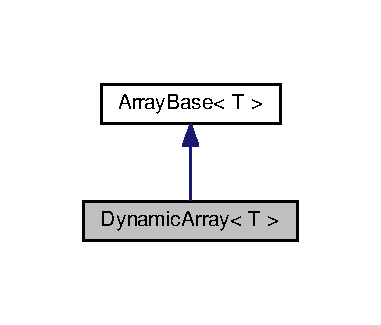
\includegraphics[width=183pt]{d1/d2b/a00018}
\end{center}
\end{figure}


Collaboration diagram for Dynamic\+Array$<$ T $>$\+:
\nopagebreak
\begin{figure}[H]
\begin{center}
\leavevmode
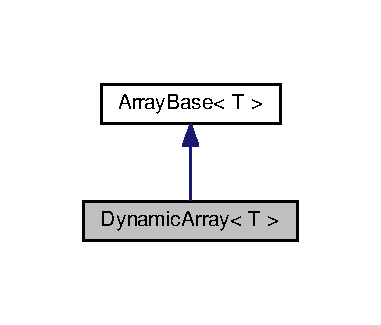
\includegraphics[width=183pt]{dd/da2/a00019}
\end{center}
\end{figure}
\subsection*{Public Member Functions}
\begin{DoxyCompactItemize}
\item 
\hyperlink{a00002_a7d42e6eaa66bab7c43f193e78d2d56a9}{Dynamic\+Array} ()
\item 
\hyperlink{a00002_a2b4e0e5f2d4af1b1ec5e37bcf2b63e27}{Dynamic\+Array} (size\+\_\+t \hyperlink{a00002_aeb1916d4d9cf7db37df86cb7a603c198}{max\+Size})
\item 
\hyperlink{a00002_ad054824baa39e43dd319dad7edff0316}{Dynamic\+Array} (size\+\_\+t \hyperlink{a00002_aeb1916d4d9cf7db37df86cb7a603c198}{max\+Size}, T \hyperlink{a00001_a6becc5e91c79d7693c0d406e466f9ec6}{fill})
\item 
\hyperlink{a00002_ae6f8273691c6c3a9284e7455e6bea18d}{Dynamic\+Array} (const \hyperlink{a00002}{Dynamic\+Array} \&arr)
\item 
\hyperlink{a00002_a1ace6a2b9a5ed8890a840c400f41ce9a}{$\sim$\+Dynamic\+Array} (void)
\item 
void \hyperlink{a00002_a7d9f29d3efa102b7d8229bfc24b9d431}{resize} (void)
\item 
void \hyperlink{a00002_aee346fa4cd0db8d1f385ea82aa93f541}{resize} (size\+\_\+t \hyperlink{a00002_aeb1916d4d9cf7db37df86cb7a603c198}{max\+Size})
\item 
const size\+\_\+t \hyperlink{a00002_aeb1916d4d9cf7db37df86cb7a603c198}{max\+Size} (void)
\item 
const \hyperlink{a00002}{Dynamic\+Array} \& \hyperlink{a00002_a683eba7c0e4652c6b1baae93e1e6ca7b}{operator=} (const \hyperlink{a00002}{Dynamic\+Array} \&)
\end{DoxyCompactItemize}
\subsection*{Additional Inherited Members}


\subsection{Detailed Description}
\subsubsection*{template$<$typename T$>$class Dynamic\+Array$<$ T $>$}

A resizable array. Inherits \hyperlink{a00001}{Array\+Base}. 

Contains specific methods to resize a raw array. \begin{DoxySince}{Since}
0.\+1.\+0 
\end{DoxySince}

\begin{DoxyTemplParams}{Template Parameters}
{\em T} & (typename) Element type of array. \\
\hline
\end{DoxyTemplParams}


Definition at line 20 of file Dynamic\+Array.\+h.



\subsection{Constructor \& Destructor Documentation}
\hypertarget{a00002_a7d42e6eaa66bab7c43f193e78d2d56a9}{\index{Dynamic\+Array@{Dynamic\+Array}!Dynamic\+Array@{Dynamic\+Array}}
\index{Dynamic\+Array@{Dynamic\+Array}!Dynamic\+Array@{Dynamic\+Array}}
\subsubsection[{Dynamic\+Array}]{\setlength{\rightskip}{0pt plus 5cm}template$<$typename T $>$ {\bf Dynamic\+Array}$<$ T $>$\+::{\bf Dynamic\+Array} (
\begin{DoxyParamCaption}
\item[{void}]{}
\end{DoxyParamCaption}
)}}\label{a00002_a7d42e6eaa66bab7c43f193e78d2d56a9}
Default initializing constructor.

Calls \hyperlink{a00001}{Array\+Base} default initializing constructor.

\begin{DoxySince}{Since}
0.\+1.\+0 
\end{DoxySince}


Definition at line 16 of file Dynamic\+Array.\+cpp.


\begin{DoxyCode}
16                                    :
17     \hyperlink{a00001}{ArrayBase<T>} ()
18 \{
19 \}
\end{DoxyCode}
\hypertarget{a00002_a2b4e0e5f2d4af1b1ec5e37bcf2b63e27}{\index{Dynamic\+Array@{Dynamic\+Array}!Dynamic\+Array@{Dynamic\+Array}}
\index{Dynamic\+Array@{Dynamic\+Array}!Dynamic\+Array@{Dynamic\+Array}}
\subsubsection[{Dynamic\+Array}]{\setlength{\rightskip}{0pt plus 5cm}template$<$typename T $>$ {\bf Dynamic\+Array}$<$ T $>$\+::{\bf Dynamic\+Array} (
\begin{DoxyParamCaption}
\item[{size\+\_\+t}]{max\+Size}
\end{DoxyParamCaption}
)}}\label{a00002_a2b4e0e5f2d4af1b1ec5e37bcf2b63e27}
Initializing constructor. Sets max size to {\ttfamily max\+Size}, effectively overriding the default.


\begin{DoxyParams}{Parameters}
{\em max\+Size} & (size\+\_\+t) Maximum size of the array. \\
\hline
\end{DoxyParams}
\begin{DoxySince}{Since}
0.\+1.\+0 
\end{DoxySince}


Definition at line 25 of file Dynamic\+Array.\+cpp.


\begin{DoxyCode}
25                                              :
26     \hyperlink{a00001}{ArrayBase<T>} (\hyperlink{a00002_aeb1916d4d9cf7db37df86cb7a603c198}{maxSize})
27 \{
28 \}
\end{DoxyCode}
\hypertarget{a00002_ad054824baa39e43dd319dad7edff0316}{\index{Dynamic\+Array@{Dynamic\+Array}!Dynamic\+Array@{Dynamic\+Array}}
\index{Dynamic\+Array@{Dynamic\+Array}!Dynamic\+Array@{Dynamic\+Array}}
\subsubsection[{Dynamic\+Array}]{\setlength{\rightskip}{0pt plus 5cm}template$<$typename T $>$ {\bf Dynamic\+Array}$<$ T $>$\+::{\bf Dynamic\+Array} (
\begin{DoxyParamCaption}
\item[{size\+\_\+t}]{max\+Size, }
\item[{T}]{fill}
\end{DoxyParamCaption}
)}}\label{a00002_ad054824baa39e43dd319dad7edff0316}
Initializing constructor. Sets max size to {\ttfamily max\+Size} and filling each element of the array with {\ttfamily fill}.


\begin{DoxyParams}{Parameters}
{\em max\+Size} & (size\+\_\+t) Maximum size of the array. \\
\hline
{\em fill} & (T) Contents of each element. \\
\hline
\end{DoxyParams}
\begin{DoxySince}{Since}
0.\+1.\+0 
\end{DoxySince}


Definition at line 34 of file Dynamic\+Array.\+cpp.


\begin{DoxyCode}
34                                                      :
35     \hyperlink{a00001}{ArrayBase<T>} (\hyperlink{a00002_aeb1916d4d9cf7db37df86cb7a603c198}{maxSize}, \hyperlink{a00001_a6becc5e91c79d7693c0d406e466f9ec6}{fill})
36 \{
37 \}
\end{DoxyCode}
\hypertarget{a00002_ae6f8273691c6c3a9284e7455e6bea18d}{\index{Dynamic\+Array@{Dynamic\+Array}!Dynamic\+Array@{Dynamic\+Array}}
\index{Dynamic\+Array@{Dynamic\+Array}!Dynamic\+Array@{Dynamic\+Array}}
\subsubsection[{Dynamic\+Array}]{\setlength{\rightskip}{0pt plus 5cm}template$<$typename T $>$ {\bf Dynamic\+Array}$<$ T $>$\+::{\bf Dynamic\+Array} (
\begin{DoxyParamCaption}
\item[{const {\bf Dynamic\+Array}$<$ T $>$ \&}]{arr}
\end{DoxyParamCaption}
)}}\label{a00002_ae6f8273691c6c3a9284e7455e6bea18d}
Copy constructor.

The source \hyperlink{a00002}{Dynamic\+Array} can be of any size, as long as they are the same type.


\begin{DoxyParams}{Parameters}
{\em arr} & (const \hyperlink{a00002}{Dynamic\+Array} \&) The source \hyperlink{a00002}{Dynamic\+Array}. \\
\hline
\end{DoxyParams}
\begin{DoxySince}{Since}
0.\+1.\+0 
\end{DoxySince}


Definition at line 43 of file Dynamic\+Array.\+cpp.


\begin{DoxyCode}
43                                                        :
44     \hyperlink{a00001}{ArrayBase<T>} (arr)
45 \{
46 \}
\end{DoxyCode}
\hypertarget{a00002_a1ace6a2b9a5ed8890a840c400f41ce9a}{\index{Dynamic\+Array@{Dynamic\+Array}!````~Dynamic\+Array@{$\sim$\+Dynamic\+Array}}
\index{````~Dynamic\+Array@{$\sim$\+Dynamic\+Array}!Dynamic\+Array@{Dynamic\+Array}}
\subsubsection[{$\sim$\+Dynamic\+Array}]{\setlength{\rightskip}{0pt plus 5cm}template$<$typename T $>$ {\bf Dynamic\+Array}$<$ T $>$\+::$\sim${\bf Dynamic\+Array} (
\begin{DoxyParamCaption}
\item[{void}]{}
\end{DoxyParamCaption}
)}}\label{a00002_a1ace6a2b9a5ed8890a840c400f41ce9a}
Destructor.

\begin{DoxySince}{Since}
0.\+1.\+0 
\end{DoxySince}


Definition at line 52 of file Dynamic\+Array.\+cpp.


\begin{DoxyCode}
53 \{
54 \}
\end{DoxyCode}


\subsection{Member Function Documentation}
\hypertarget{a00002_aeb1916d4d9cf7db37df86cb7a603c198}{\index{Dynamic\+Array@{Dynamic\+Array}!max\+Size@{max\+Size}}
\index{max\+Size@{max\+Size}!Dynamic\+Array@{Dynamic\+Array}}
\subsubsection[{max\+Size}]{\setlength{\rightskip}{0pt plus 5cm}template$<$typename T $>$ const size\+\_\+t {\bf Dynamic\+Array}$<$ T $>$\+::max\+Size (
\begin{DoxyParamCaption}
\item[{void}]{}
\end{DoxyParamCaption}
)}}\label{a00002_aeb1916d4d9cf7db37df86cb7a603c198}
Query the maximum size of the array.


\begin{DoxyParams}{Parameters}
{\em (void)} & \\
\hline
\end{DoxyParams}
\begin{DoxySince}{Since}
0.\+1.\+0 
\end{DoxySince}


Definition at line 106 of file Dynamic\+Array.\+cpp.


\begin{DoxyCode}
107 \{
108     \textcolor{keywordflow}{return} this->\_maxSize;
109 \}
\end{DoxyCode}
\hypertarget{a00002_a683eba7c0e4652c6b1baae93e1e6ca7b}{\index{Dynamic\+Array@{Dynamic\+Array}!operator=@{operator=}}
\index{operator=@{operator=}!Dynamic\+Array@{Dynamic\+Array}}
\subsubsection[{operator=}]{\setlength{\rightskip}{0pt plus 5cm}template$<$typename T $>$ const {\bf Dynamic\+Array}$<$ T $>$ \& {\bf Dynamic\+Array}$<$ T $>$\+::operator= (
\begin{DoxyParamCaption}
\item[{const {\bf Dynamic\+Array}$<$ T $>$ \&}]{rhs}
\end{DoxyParamCaption}
)}}\label{a00002_a683eba7c0e4652c6b1baae93e1e6ca7b}
Assignment operator.

Assigns the right hand side of the assignment operator to the left. 
\begin{DoxyParams}{Parameters}
{\em rhs} & (const \hyperlink{a00002}{Dynamic\+Array} \&) The source \hyperlink{a00002}{Dynamic\+Array}. \\
\hline
\end{DoxyParams}
\begin{DoxySince}{Since}
0.\+1.\+0 
\end{DoxySince}


Definition at line 115 of file Dynamic\+Array.\+cpp.


\begin{DoxyCode}
115                                                                               \{
116     \textcolor{comment}{// Check for self-assignment. If self-assigned, return the pointer}
117     \textcolor{keywordflow}{if} (\textcolor{keyword}{this} == &rhs) \{
118         \textcolor{keywordflow}{return} *\textcolor{keyword}{this};
119     \}
120 
121     \textcolor{comment}{// Resize this to match rhs}
122     \textcolor{keywordflow}{if} (this->\hyperlink{a00002_aeb1916d4d9cf7db37df86cb7a603c198}{maxSize}() != rhs.\hyperlink{a00002_aeb1916d4d9cf7db37df86cb7a603c198}{maxSize}()) \{
123         this->\hyperlink{a00002_a7d9f29d3efa102b7d8229bfc24b9d431}{resize}(rhs.\hyperlink{a00002_aeb1916d4d9cf7db37df86cb7a603c198}{maxSize}());
124     \}
125 
126     \textcolor{comment}{// Copy all elements from rhs to this}
127     \textcolor{keywordflow}{for} (\textcolor{keywordtype}{size\_t} i = 0; i < rhs.\hyperlink{a00001_aeed263e1e987901c8cc2c1e1d3102d73}{size}(); i++) \{
128         this->\hyperlink{a00001_a5a9fe61509061defe530d0ebc3a91497}{set}(i, rhs.\hyperlink{a00001_aabda9501caf50b75ce09e7ef47fd1de7}{get}(i));
129     \}
130 
131     \textcolor{keywordflow}{return} *\textcolor{keyword}{this};
132 \}
\end{DoxyCode}
\hypertarget{a00002_a7d9f29d3efa102b7d8229bfc24b9d431}{\index{Dynamic\+Array@{Dynamic\+Array}!resize@{resize}}
\index{resize@{resize}!Dynamic\+Array@{Dynamic\+Array}}
\subsubsection[{resize}]{\setlength{\rightskip}{0pt plus 5cm}template$<$typename T $>$ void {\bf Dynamic\+Array}$<$ T $>$\+::resize (
\begin{DoxyParamCaption}
\item[{void}]{}
\end{DoxyParamCaption}
)}}\label{a00002_a7d9f29d3efa102b7d8229bfc24b9d431}
Sets max\+Size equal to current\+Size.


\begin{DoxyParams}{Parameters}
{\em (void)} & \\
\hline
\end{DoxyParams}
\begin{DoxySince}{Since}
0.\+1.\+0 
\end{DoxySince}


Definition at line 60 of file Dynamic\+Array.\+cpp.


\begin{DoxyCode}
61 \{
62     this->\hyperlink{a00002_a7d9f29d3efa102b7d8229bfc24b9d431}{resize}(this->\hyperlink{a00001_aeed263e1e987901c8cc2c1e1d3102d73}{size}());
63 \}
\end{DoxyCode}
\hypertarget{a00002_aee346fa4cd0db8d1f385ea82aa93f541}{\index{Dynamic\+Array@{Dynamic\+Array}!resize@{resize}}
\index{resize@{resize}!Dynamic\+Array@{Dynamic\+Array}}
\subsubsection[{resize}]{\setlength{\rightskip}{0pt plus 5cm}template$<$typename T $>$ void {\bf Dynamic\+Array}$<$ T $>$\+::resize (
\begin{DoxyParamCaption}
\item[{size\+\_\+t}]{max\+Size}
\end{DoxyParamCaption}
)}}\label{a00002_aee346fa4cd0db8d1f385ea82aa93f541}
Sets a new max\+Size.

If max\+Size is less than \+\_\+current\+Size, then the array is truncated. If max\+Size is greater than current\+Size, then the array is made larger and the new elements are not initialized to anything. If max\+Size is the same as current\+Size, then nothing happens except for the removal of uninitialized elements.


\begin{DoxyParams}{Parameters}
{\em max\+Size} & The new maximum size of the array. \\
\hline
\end{DoxyParams}
\begin{DoxySince}{Since}
0.\+1.\+0 
\end{DoxySince}


Definition at line 69 of file Dynamic\+Array.\+cpp.


\begin{DoxyCode}
70 \{
71 
72     \textcolor{keywordflow}{if} (this->\hyperlink{a00001_aeed263e1e987901c8cc2c1e1d3102d73}{size}() >= \hyperlink{a00002_aeb1916d4d9cf7db37df86cb7a603c198}{maxSize}) \{
73         this->\_currentSize = \hyperlink{a00002_aeb1916d4d9cf7db37df86cb7a603c198}{maxSize};
74         this->\_maxSize = \hyperlink{a00002_aeb1916d4d9cf7db37df86cb7a603c198}{maxSize};
75     \} \textcolor{keywordflow}{else} \{
76         \textcolor{comment}{/* Create tempArray to put existing elements in this->\_data, setting}
77 \textcolor{comment}{         * the size of the tempArray to param new\_size.}
78 \textcolor{comment}{         */}
79         T * tempArray = \textcolor{keyword}{new} T[\hyperlink{a00002_aeb1916d4d9cf7db37df86cb7a603c198}{maxSize}];
80 
81         \textcolor{comment}{// Copy contents of this->\_data to tempArray one element at a time.}
82         \textcolor{keywordtype}{size\_t} i = 0;
83         \textcolor{keywordflow}{while} (i < \hyperlink{a00002_aeb1916d4d9cf7db37df86cb7a603c198}{maxSize} && i < this->\hyperlink{a00001_aeed263e1e987901c8cc2c1e1d3102d73}{size}()) \{
84             tempArray[i] = this->\textcolor{keyword}{get}(i);
85             i++;
86         \}
87 
88         \textcolor{keywordflow}{if} (this->\_data == &tempArray) \{
89             \textcolor{comment}{// Destroy old raw array.}
90             \textcolor{keyword}{delete} [] this->\_data;
91         \} \textcolor{keywordflow}{else} \{
92             std::runtime\_error(\textcolor{stringliteral}{"Array resize failed."});
93         \}
94 
95         \textcolor{comment}{// Assign tempArray to this->\_data.}
96         this->\_data = tempArray;
97         
98         this->\_maxSize = \hyperlink{a00002_aeb1916d4d9cf7db37df86cb7a603c198}{maxSize};
99     \}
100 \}
\end{DoxyCode}


The documentation for this class was generated from the following files\+:\begin{DoxyCompactItemize}
\item 
/home/bdfoster/\+Projects/c++/templates/\hyperlink{a00006}{Dynamic\+Array.\+h}\item 
/home/bdfoster/\+Projects/c++/templates/\hyperlink{a00005}{Dynamic\+Array.\+cpp}\end{DoxyCompactItemize}

\chapter{File Documentation}
\hypertarget{a00003}{\section{/home/bdfoster/\+Projects/c++/templates/\+Array\+Base.cpp File Reference}
\label{a00003}\index{/home/bdfoster/\+Projects/c++/templates/\+Array\+Base.\+cpp@{/home/bdfoster/\+Projects/c++/templates/\+Array\+Base.\+cpp}}
}
{\ttfamily \#include \char`\"{}Array\+Base.\+h\char`\"{}}\\*
{\ttfamily \#include $<$stdexcept$>$}\\*
Include dependency graph for Array\+Base.\+cpp\+:
\nopagebreak
\begin{figure}[H]
\begin{center}
\leavevmode
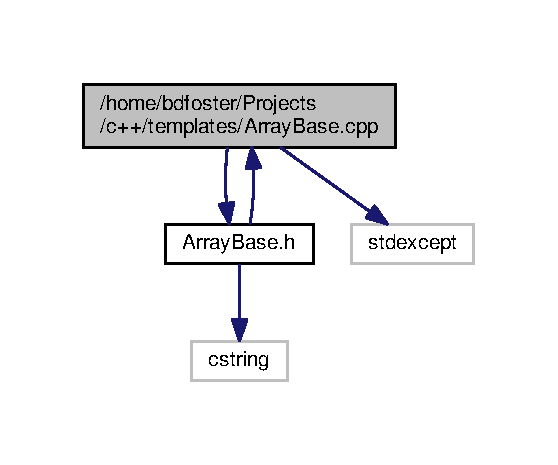
\includegraphics[width=268pt]{de/d5e/a00007}
\end{center}
\end{figure}
This graph shows which files directly or indirectly include this file\+:
\nopagebreak
\begin{figure}[H]
\begin{center}
\leavevmode
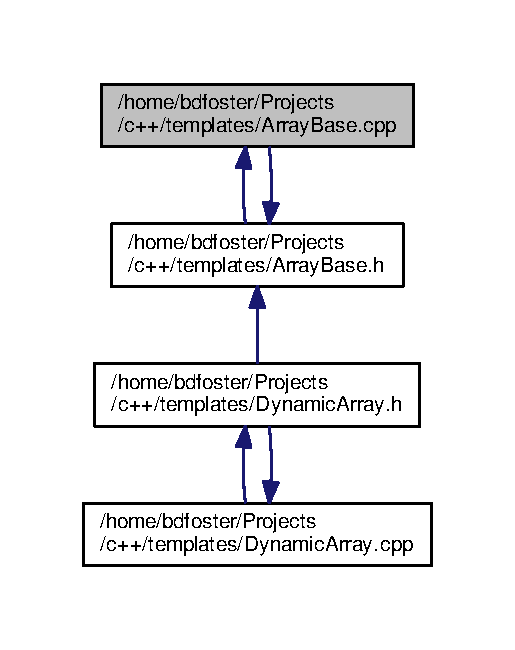
\includegraphics[width=247pt]{d4/dee/a00008}
\end{center}
\end{figure}
\subsection*{Macros}
\begin{DoxyCompactItemize}
\item 
\#define \hyperlink{a00003_aeb58186c19f02cd09f0d5295a03a8a87}{\+\_\+\+A\+R\+R\+A\+Y\+\_\+\+B\+A\+S\+E\+\_\+\+C\+P\+P\+\_\+}
\end{DoxyCompactItemize}


\subsection{Detailed Description}
\begin{DoxyAuthor}{Author}
Brian D. Foster 
\end{DoxyAuthor}
\begin{DoxyCopyright}{Copyright}
The M\+I\+T License (M\+I\+T) 
\end{DoxyCopyright}


Definition in file \hyperlink{a00003_source}{Array\+Base.\+cpp}.



\subsection{Macro Definition Documentation}
\hypertarget{a00003_aeb58186c19f02cd09f0d5295a03a8a87}{\index{Array\+Base.\+cpp@{Array\+Base.\+cpp}!\+\_\+\+A\+R\+R\+A\+Y\+\_\+\+B\+A\+S\+E\+\_\+\+C\+P\+P\+\_\+@{\+\_\+\+A\+R\+R\+A\+Y\+\_\+\+B\+A\+S\+E\+\_\+\+C\+P\+P\+\_\+}}
\index{\+\_\+\+A\+R\+R\+A\+Y\+\_\+\+B\+A\+S\+E\+\_\+\+C\+P\+P\+\_\+@{\+\_\+\+A\+R\+R\+A\+Y\+\_\+\+B\+A\+S\+E\+\_\+\+C\+P\+P\+\_\+}!Array\+Base.\+cpp@{Array\+Base.\+cpp}}
\subsubsection[{\+\_\+\+A\+R\+R\+A\+Y\+\_\+\+B\+A\+S\+E\+\_\+\+C\+P\+P\+\_\+}]{\setlength{\rightskip}{0pt plus 5cm}\#define \+\_\+\+A\+R\+R\+A\+Y\+\_\+\+B\+A\+S\+E\+\_\+\+C\+P\+P\+\_\+}}\label{a00003_aeb58186c19f02cd09f0d5295a03a8a87}


Definition at line 8 of file Array\+Base.\+cpp.


\hypertarget{a00004}{\section{/home/bdfoster/\+Projects/c++/templates/\+Array\+Base.h File Reference}
\label{a00004}\index{/home/bdfoster/\+Projects/c++/templates/\+Array\+Base.\+h@{/home/bdfoster/\+Projects/c++/templates/\+Array\+Base.\+h}}
}
{\ttfamily \#include $<$cstring$>$}\\*
{\ttfamily \#include \char`\"{}Array\+Base.\+cpp\char`\"{}}\\*
Include dependency graph for Array\+Base.\+h\+:
\nopagebreak
\begin{figure}[H]
\begin{center}
\leavevmode
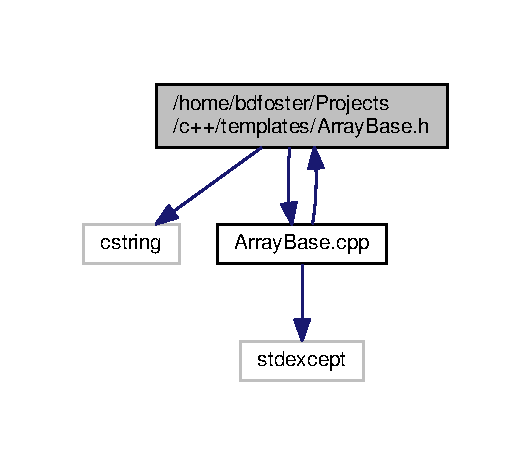
\includegraphics[width=255pt]{da/da0/a00009}
\end{center}
\end{figure}
This graph shows which files directly or indirectly include this file\+:
\nopagebreak
\begin{figure}[H]
\begin{center}
\leavevmode
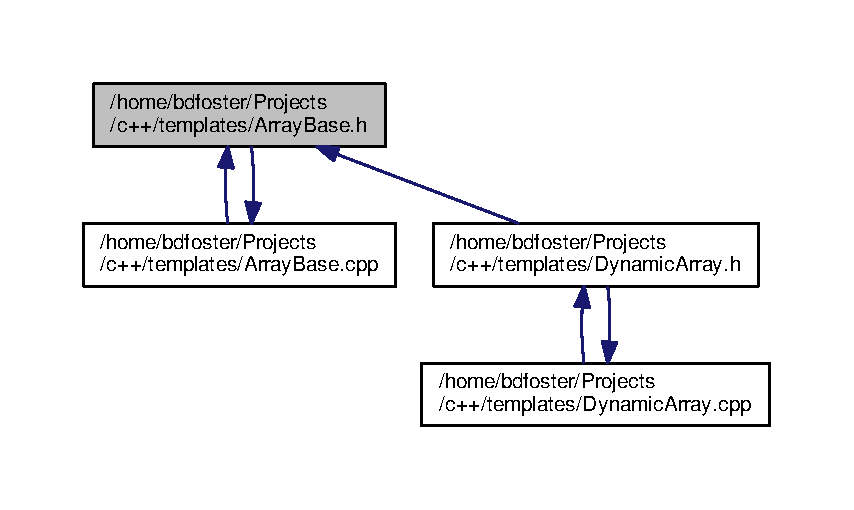
\includegraphics[width=350pt]{d7/dec/a00010}
\end{center}
\end{figure}
\subsection*{Classes}
\begin{DoxyCompactItemize}
\item 
class \hyperlink{a00001}{Array\+Base$<$ T $>$}
\begin{DoxyCompactList}\small\item\em Base class for array-\/like structures. \end{DoxyCompactList}\end{DoxyCompactItemize}


\subsection{Detailed Description}
\begin{DoxyAuthor}{Author}
Brian D. Foster 
\end{DoxyAuthor}
\begin{DoxyCopyright}{Copyright}
The M\+I\+T License (M\+I\+T) 
\end{DoxyCopyright}


Definition in file \hyperlink{a00004_source}{Array\+Base.\+h}.


\hypertarget{a00005}{\section{/home/bdfoster/\+Projects/c++/templates/\+Dynamic\+Array.cpp File Reference}
\label{a00005}\index{/home/bdfoster/\+Projects/c++/templates/\+Dynamic\+Array.\+cpp@{/home/bdfoster/\+Projects/c++/templates/\+Dynamic\+Array.\+cpp}}
}
{\ttfamily \#include \char`\"{}Dynamic\+Array.\+h\char`\"{}}\\*
Include dependency graph for Dynamic\+Array.\+cpp\+:
\nopagebreak
\begin{figure}[H]
\begin{center}
\leavevmode
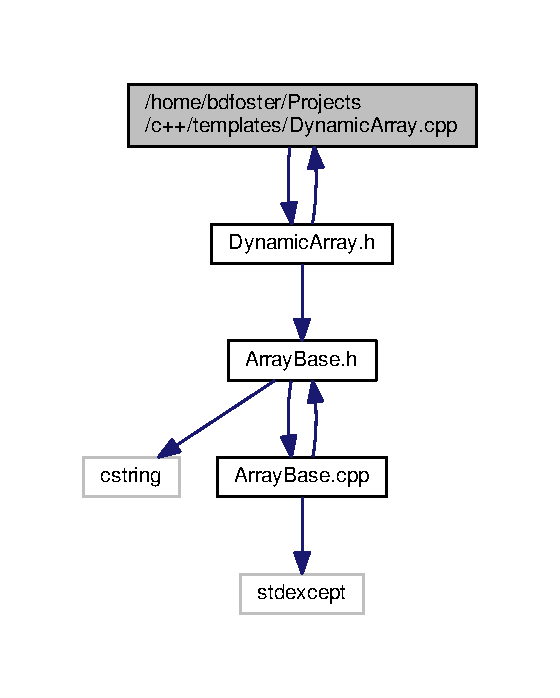
\includegraphics[width=269pt]{da/d45/a00011}
\end{center}
\end{figure}
This graph shows which files directly or indirectly include this file\+:
\nopagebreak
\begin{figure}[H]
\begin{center}
\leavevmode
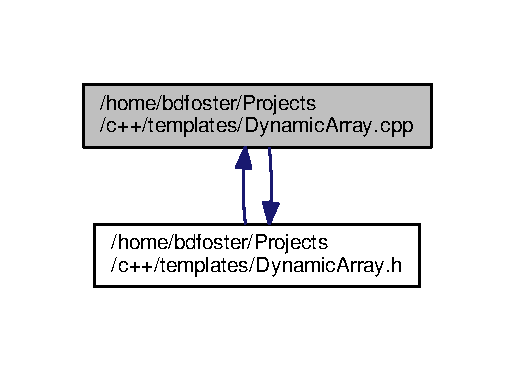
\includegraphics[width=247pt]{df/d86/a00012}
\end{center}
\end{figure}
\subsection*{Macros}
\begin{DoxyCompactItemize}
\item 
\#define \hyperlink{a00005_a2456e0218e200f6ae1142d51cbbc0941}{\+\_\+\+D\+Y\+N\+A\+M\+I\+C\+\_\+\+A\+R\+R\+A\+Y\+\_\+\+C\+P\+P\+\_\+}
\end{DoxyCompactItemize}


\subsection{Detailed Description}
\begin{DoxyAuthor}{Author}
Brian D. Foster 
\end{DoxyAuthor}
\begin{DoxyCopyright}{Copyright}
The M\+I\+T License (M\+I\+T) 
\end{DoxyCopyright}


Definition in file \hyperlink{a00005_source}{Dynamic\+Array.\+cpp}.



\subsection{Macro Definition Documentation}
\hypertarget{a00005_a2456e0218e200f6ae1142d51cbbc0941}{\index{Dynamic\+Array.\+cpp@{Dynamic\+Array.\+cpp}!\+\_\+\+D\+Y\+N\+A\+M\+I\+C\+\_\+\+A\+R\+R\+A\+Y\+\_\+\+C\+P\+P\+\_\+@{\+\_\+\+D\+Y\+N\+A\+M\+I\+C\+\_\+\+A\+R\+R\+A\+Y\+\_\+\+C\+P\+P\+\_\+}}
\index{\+\_\+\+D\+Y\+N\+A\+M\+I\+C\+\_\+\+A\+R\+R\+A\+Y\+\_\+\+C\+P\+P\+\_\+@{\+\_\+\+D\+Y\+N\+A\+M\+I\+C\+\_\+\+A\+R\+R\+A\+Y\+\_\+\+C\+P\+P\+\_\+}!Dynamic\+Array.\+cpp@{Dynamic\+Array.\+cpp}}
\subsubsection[{\+\_\+\+D\+Y\+N\+A\+M\+I\+C\+\_\+\+A\+R\+R\+A\+Y\+\_\+\+C\+P\+P\+\_\+}]{\setlength{\rightskip}{0pt plus 5cm}\#define \+\_\+\+D\+Y\+N\+A\+M\+I\+C\+\_\+\+A\+R\+R\+A\+Y\+\_\+\+C\+P\+P\+\_\+}}\label{a00005_a2456e0218e200f6ae1142d51cbbc0941}


Definition at line 8 of file Dynamic\+Array.\+cpp.


\hypertarget{a00006}{\section{/home/bdfoster/\+Projects/c++/templates/\+Dynamic\+Array.h File Reference}
\label{a00006}\index{/home/bdfoster/\+Projects/c++/templates/\+Dynamic\+Array.\+h@{/home/bdfoster/\+Projects/c++/templates/\+Dynamic\+Array.\+h}}
}
{\ttfamily \#include \char`\"{}Array\+Base.\+h\char`\"{}}\\*
{\ttfamily \#include \char`\"{}Dynamic\+Array.\+cpp\char`\"{}}\\*
Include dependency graph for Dynamic\+Array.\+h\+:
\nopagebreak
\begin{figure}[H]
\begin{center}
\leavevmode
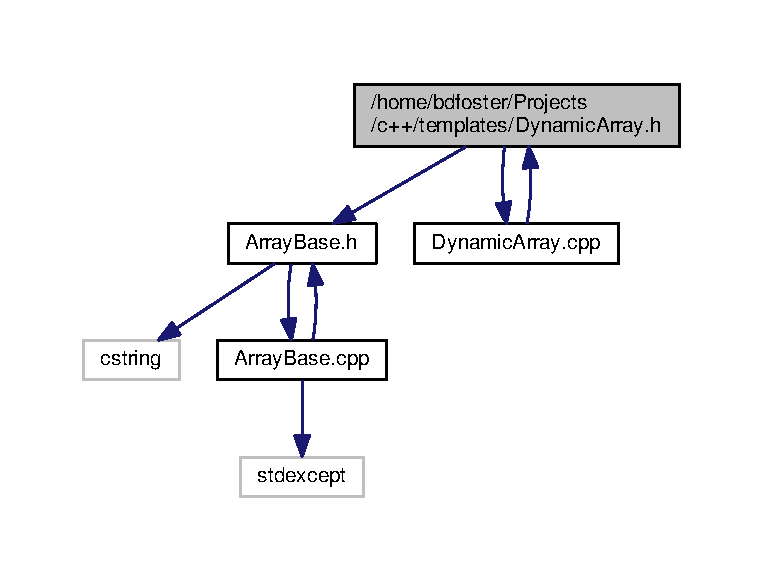
\includegraphics[width=350pt]{d7/dd4/a00013}
\end{center}
\end{figure}
This graph shows which files directly or indirectly include this file\+:
\nopagebreak
\begin{figure}[H]
\begin{center}
\leavevmode
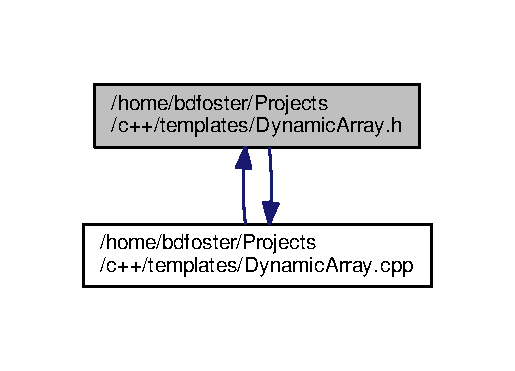
\includegraphics[width=247pt]{d2/de7/a00014}
\end{center}
\end{figure}
\subsection*{Classes}
\begin{DoxyCompactItemize}
\item 
class \hyperlink{a00002}{Dynamic\+Array$<$ T $>$}
\begin{DoxyCompactList}\small\item\em A resizable array. Inherits \hyperlink{a00001}{Array\+Base}. \end{DoxyCompactList}\end{DoxyCompactItemize}


\subsection{Detailed Description}
\begin{DoxyAuthor}{Author}
Brian D. Foster 
\end{DoxyAuthor}
\begin{DoxyCopyright}{Copyright}
The M\+I\+T License (M\+I\+T) 
\end{DoxyCopyright}


Definition in file \hyperlink{a00006_source}{Dynamic\+Array.\+h}.


%--- End generated contents ---

% Index
\newpage
\phantomsection
\addcontentsline{toc}{chapter}{Index}
\printindex

\end{document}
